%%%%%%%%%%%%%%%%%%%%%%%%%%%%%%%%%%%%%%%%%%%%%%%%%%%%%%%%
%%%%                                              %%%%%%
%%%%  Author: Peter Wilson                        %%%%%%
%%%%                                              %%%%%%
%%%%  Background of shells                        %%%%%%
%%%%                                              %%%%%%
%%%%%%%%%%%%%%%%%%%%%%%%%%%%%%%%%%%%%%%%%%%%%%%%%%%%%%%%

\chapter{DSG technology derivation}
\label{app:DSG technology derivation}

The DSG element technology aims to mitigate shear locking in 5-parameter based shell formulations via the concept of discrete shear gaps. This term, coined by Bletzinger et al. \cite{Ble00}, refers to the difference in transverse displacements between a pure 3-parameter Kirchhoff formulation and a 5-parameter Reissner-Mindlin formulation. More explicitly, this concept can be illustrated by considering the deformation of a beam:



FORMULATION LAYOUT AS PER BLETZINGER IN \cite{Ble00}, PICTURE FROM SMOOTHED DSG PAPER 

\begin{figure}[H]
	\centering
	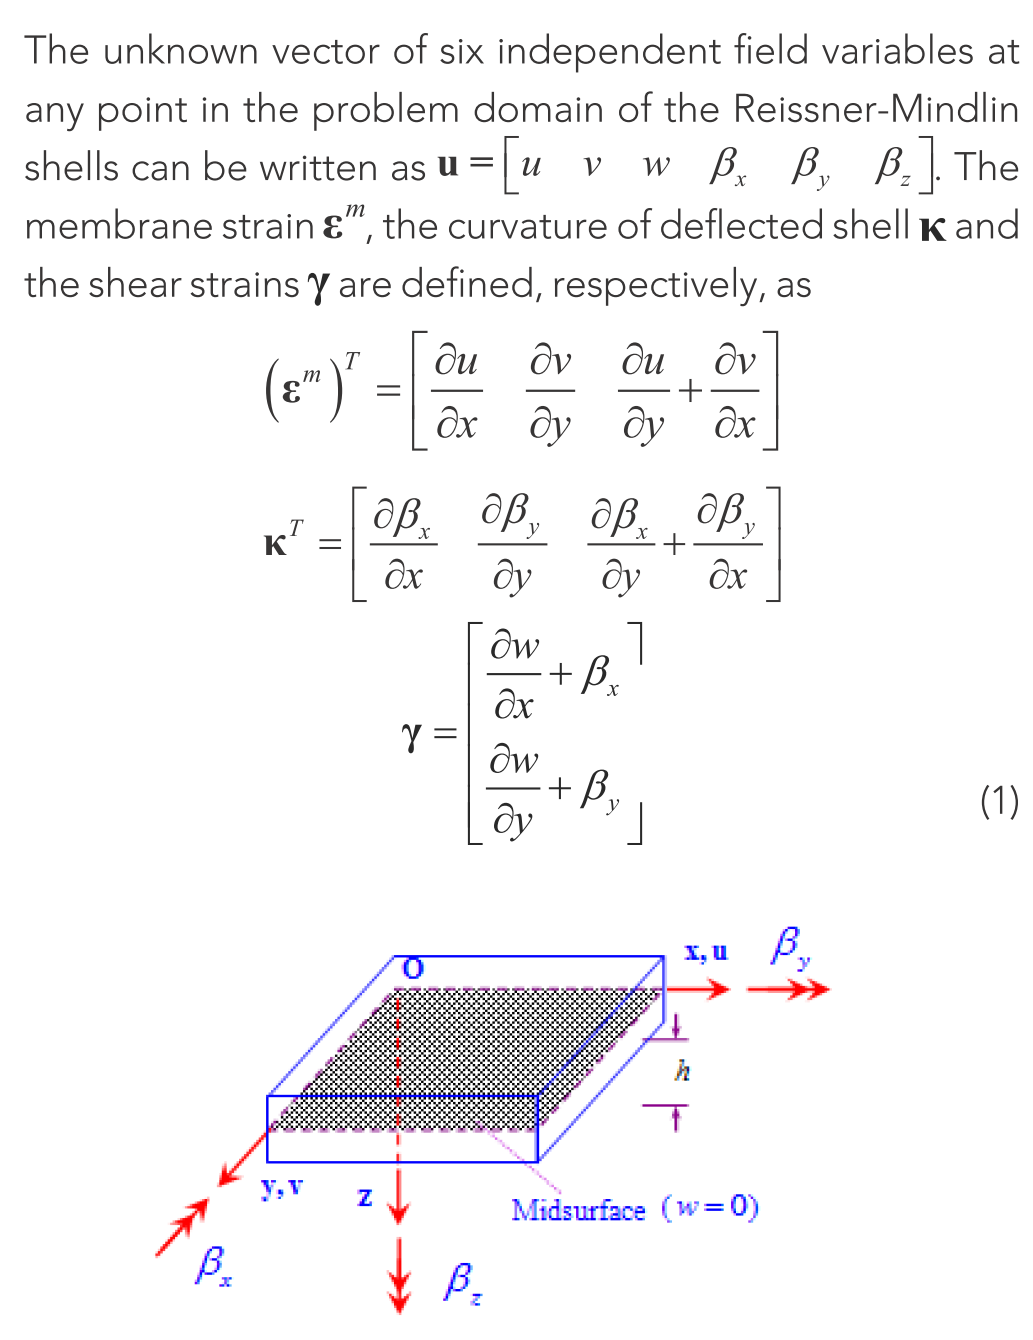
\includegraphics[height=10cm]{images/dsg_derivation_CS_layout}
	\caption{DSG system setup as per Bletzinger}
	\label{fig:dsgderivationcslayout}
\end{figure}

\begin{figure}[H]
	\centering
	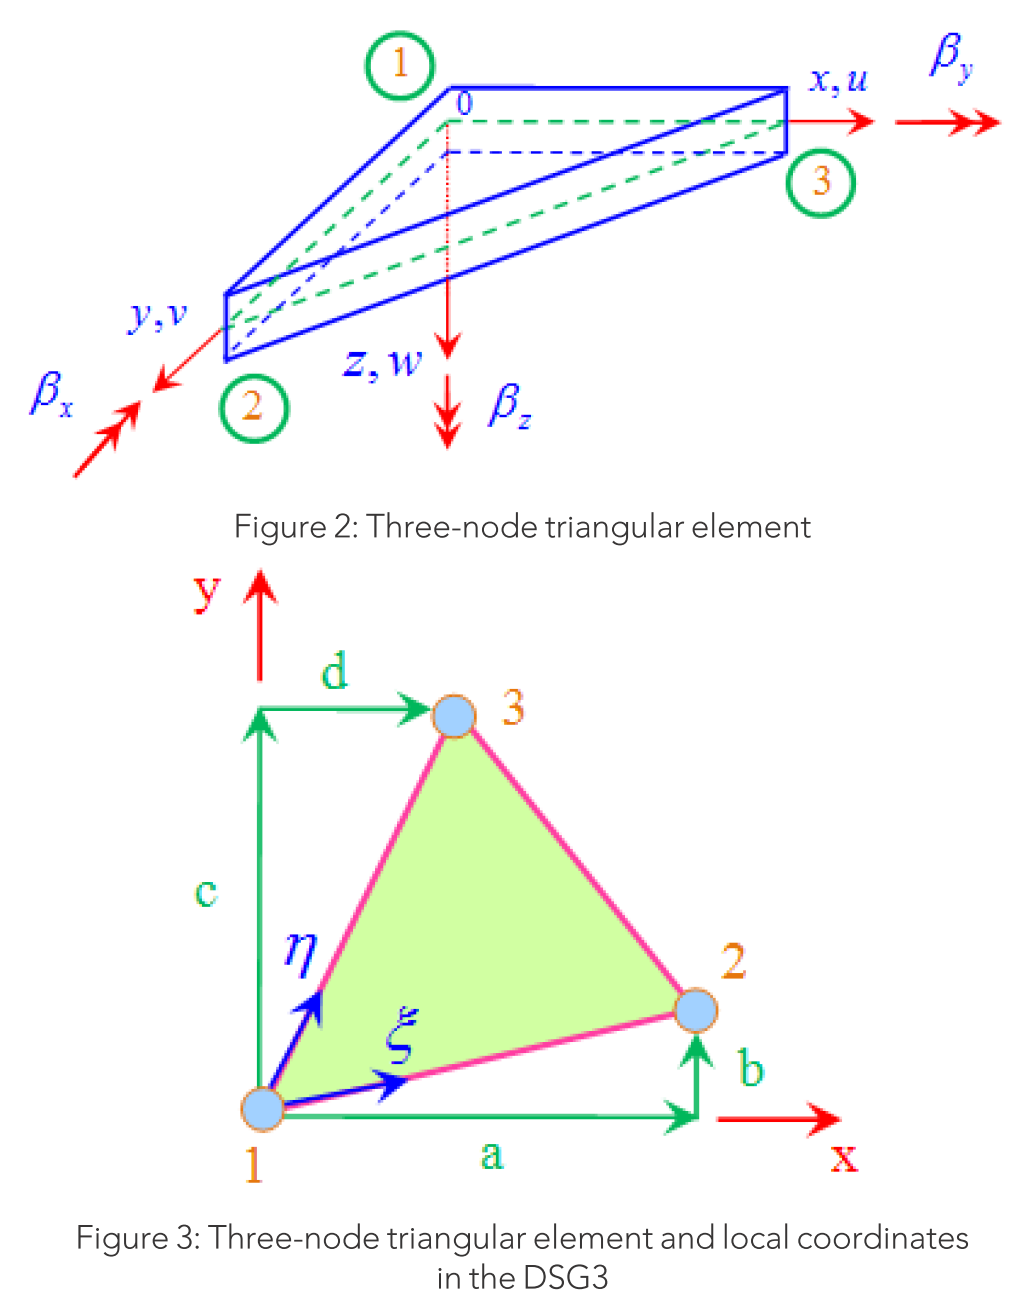
\includegraphics[height=10cm]{images/dsg_derivation_CS_layout2}
	\caption{DSG system setup as per Bletzinger}
	\label{fig:dsgderivationcslayout2}
\end{figure}

THIS GIVES THE FOLLOWING B MATRIX:
\begin{figure}[H]
	\centering
	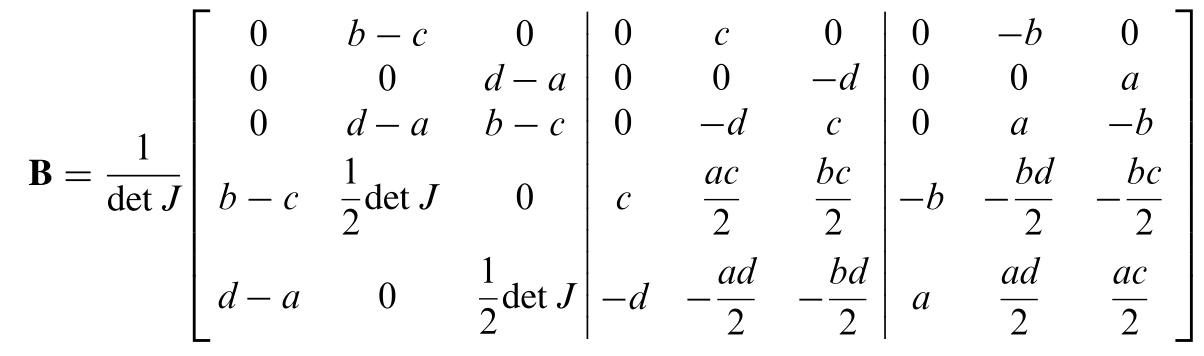
\includegraphics[width=8cm]{images/dsg_derivation_bletzy_Bmat.png}
	\caption{DSG Bmat as per Bletzinger}
	\label{fig:dsgderivationcslayout3}
\end{figure}


HOWEVER, ROTATIONS IN KRATOS ARE DEFINED AS GENERAL NODAL ROTATIONS FOLLOWING RIGHT HAND SCREW RULE, THUS.

$R_x = \beta_y$
$R_y = -\beta_x$
\begin{figure}[H]
	\centering
	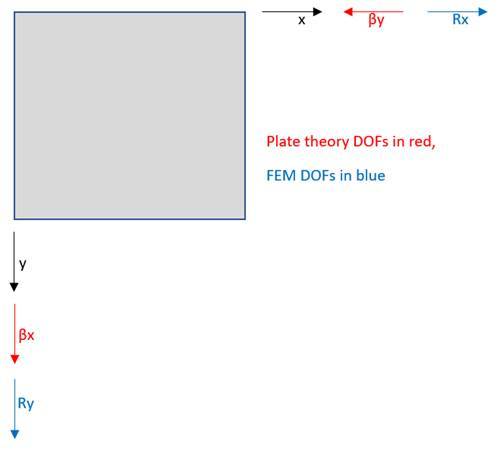
\includegraphics[width=8cm]{images/dsg_derivation_DOF_conversion.png}
	\caption{DOF conversion}
	\label{fig:dsgderivationcslayout4}
\end{figure}

